\documentclass[10pt]{article}

\usepackage{listings}
\usepackage[utf8]{inputenc}
\usepackage{fancyvrb}
\usepackage{graphicx}
\PassOptionsToPackage{hyphens}{url}\usepackage{hyperref}

\graphicspath{ {./Imagenes/} }

\lstset{
}

\begin{document}
\pagenumbering{arabic}

\Large
 \begin{center}
Algoritmia para problemas difíciles\\ 
\small  
1. Problemas intratables\\

\hspace{10pt}

\large
Pablo Noel Carreras Aguerri\\
\small
718743\\

\end{center}

\normalsize

\vspace{10mm}

\noindent
\textbf{Ejercicio 4} Demostrar que los siguientes problemas están en NP:

\begin{enumerate}
	\item El grafo G tiene un camino simple (es decir, sin repetir vértices) de longitud k?
	\item Es n un entero compuesto (es decir, no es primo)?
	\item Tiene un grafo G una cobertura de vértices de tamaño k?
\end{enumerate}

\vspace{10mm}

\noindent
\textbf{Respuestas}\\

Para demostrar la pertenencia de los distintos problemas a NP, se va a proceder a la reducción de un problema conocido de NP a cada uno de los problemas planteados:

\begin{enumerate}

	\item Para empezar, la primera similitud obvia del problema es con un camino hamiltoniano, el cual es un caso particular del problema en el que k es igual al número de vértices del grafo G. Por esto, el objetivo principal sería reducir el problema de ciclo hamiltoniano a camino hamiltoniano. De esta manera quedaría demostrado que el problema pertenece a NP (Ciclo hamiltoniano es un problema conocido de NP).\\

	La reducción se basa en el siguiente razonamiento: partiendo del grafo G, se selecciona una arista aleatoria y en ambos vértices de esta se añade un nodo adicional, obtenieniendo así el grafo G'. Si ahora se busca un camino hamiltoniano sobre este nuevo grafo, en caso de existir, este empezará y acabara en uno de los nuevos nodos añadidos (el caso contrario implica que no existe un camino hamiltoniano para el grafo).\\
		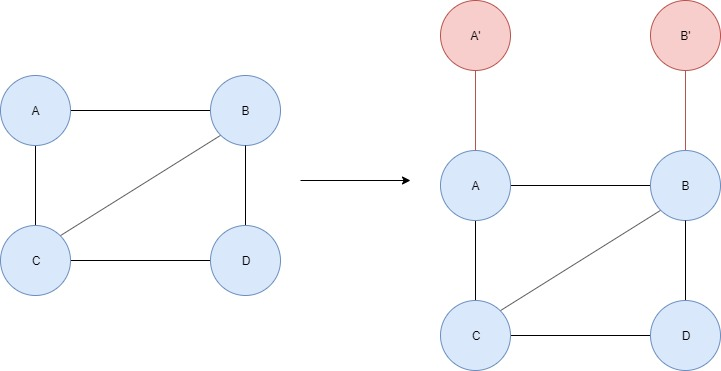
\includegraphics[width=\textwidth]{grafo3.jpg}

	Así pues, si pasamos al problema planteado como argumentos un grafo transformado G' y "k=número de vértices", si la salida confirma la existencia de un camino hamiltoniano para el grafo G' lo haría consecuentemente para la del ciclo hamiltoniano en el grafo G. Así pues un bucle que inspeccionase linealmente cada par de vértices consecutivos resolvería el problema de ciclo hamiltoniano. Queda así demostrado que el problema está en NP, ya que lo contrario supondría negar que el problema de ciclo hamiltoniano no está en NP.\\

	*La reducción de ciclo a camino hamiltoniano usada está inspirada en foros y ejercicios de Internet como los de los siguientes enlaces: \url{https://math.stackexchange.com/questions/7130/reduction-from-hamiltonian-cycle-to-hamiltonian-path}, \url{https://personal.vu.nl/l.stougie/Courses/COB/AntwoordenCT.pdf}\\

	\item El problema al que se va a asemejar la búsqueda de números primos es a SAT. La semejanza planteada se basa en la visión de los números como conjuntos de n bits. De esta manera, se puede plantear un circuito con un multiplicador y un comparador, el cual tiene una expresión booleana correspondiente.\\
		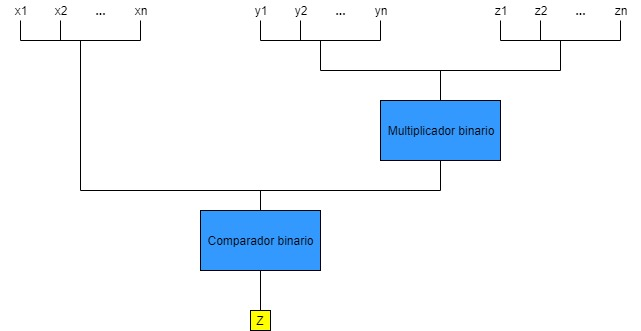
\includegraphics[width=\textwidth]{circuito.jpg}

	Los números verdaderamente consideradas como entrada son \textit{y} y \textit{z}, ya que \textit{x} sería una constante fijada al equivalente en bits al número cuya \textit{"primalidad"} se quiere comprobar. Así pues, encontrar el número a través de SAT es sencillo, pero ineficiente dentro del orden de los problemas NP. De la misma manera es también sencillo introducir con el cambio inverso la entrada del SAT en el problema planteado. Queda pues clado que la comprobación de \textit{"primality"} es un problema de NP, ya que ambos se pueden reducir el uno al otro.\\
	
	\item Al igual que con el anterior, se puede hacer una reducción desde SAT e incluso del caso particular 3-SAT. Para esto hay que contemplar los grafos como matrices de adyacencia (que además es una matriz  cuadrada). Partiendo de esto, se puede plantear un circuito de SAT consistente en una linea de ORs y otra de ANDs. Por ejemplo, para un grafo con dos vértices unidos y su matriz de adyacencia "M{ [0, 1], [1, 0] }", se plantea la expresión: (M[0][1] and M[1][0]). Conforme el tamaño aumenta el número de entradas de la and es igual al número de filas (que es igual al de columnas) y todas ellas van a parar a una puerta OR. Así pues, este problema es reducible a 3-SAT y viceversa de forma sencilla. Esto demuestra que el problema pertenece a NP.


\end{enumerate}

\end{document}